\documentclass[12pt]{beamer}
\usepackage[utf8]{inputenc}
\usepackage[T1]{fontenc}
\usepackage{lmodern}
\usepackage[english]{babel}
\usepackage{amsmath}
\usepackage{amsfonts}
\usepackage{amssymb}
\usepackage{graphicx}
\usetheme{default}
\begin{document}
	\addtocounter{framenumber}{-1}
	
	\author{Sewade Ogun}
	\title{Adversarial Examples}
	\subtitle{A new evil has announced its arrival...}
	%\logo{}
	\institute{{\normalsize AMMI, AIMS Ghana}}
	\date{\today}
	%\subject{}
	%\setbeamercovered{transparent}
	%\setbeamertemplate{navigation symbols}{}
	\begin{frame}[plain]
	\maketitle
	\begin{figure}
		\centering
		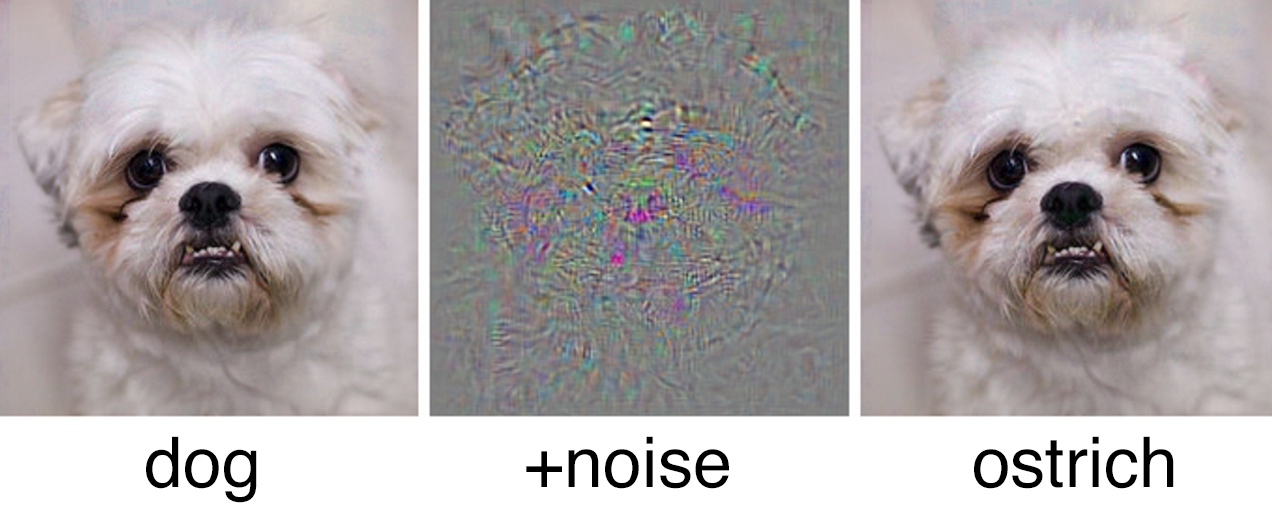
\includegraphics[width=0.85\linewidth,height=0.4\textheight]{img/dog}
		\label{fig:dog}
	\end{figure}
\end{frame}

\section{Objectives}
\begin{frame}
\frametitle{Objectives}
\begin{enumerate}
	\item To show the effect and effectiveness of adversarial examples in machine learning predictions
	\item To understand the adversary, and determine how to combat it.
	\item To enlighten the audience on machine learning security.
\end{enumerate}

\end{frame}

\begin{frame}
	\frametitle{Outlines}
	\tableofcontents
\end{frame}

\section{Introduction}
\begin{frame}
\frametitle{Introduction}
	\begin{itemize}
		\item[o] An \textbf{adversarial example} is an instance with small, intentional feature perturbations that cause a machine learning model to make a false prediction.\protect\footnotemark
		\footnotetext{https://christophm.github.io/interpretable-ml-book/adversarial.html}
		
		\item[o] A type of \textbf{counterfactual example}
		
		\begin{figure}
			\centering
			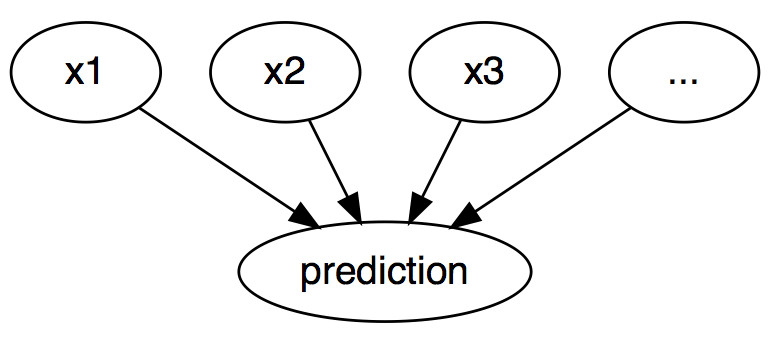
\includegraphics[width=0.7\linewidth,height=0.3\textheight]{img/graph}
			\caption{Causal relationships between inputs of a machine learning model and the predictions}
			\label{fig:graph}
		\end{figure}
		
	\end{itemize}
	
\end{frame}

\section{Properties of Counterfactual Instance}
\begin{frame}
\frametitle{Properties of Counterfactual Instance}
A counterfactual should;
\begin{itemize}
	\item[o] be as \textbf{similar} as possible to the instance regarding feature values \pause
	\item[o] change as \textbf{few} features as possible. \pause
	\item[o] have feature values that are \textbf{likely}. \pause
	\item[o] produce the predefined prediction as \textbf{closely} as possible.
\end{itemize}
\end{frame}


\section{Examples}
\begin{frame}
\frametitle{Examples}
\begin{enumerate}
	\item You submit your details for an offer in such a way that the machine classify you as eligible. \pause
	\item A spam detector by-passed \pause
	\item Object counterfeit - knife as umbrella \pause
	\item Self-driving cars can be deceived by images to misclassify stop-signs.
\end{enumerate}
\end{frame}

\subsection{Techniques}
\begin{frame}
\frametitle{Techniques}
\begin{enumerate}
	\item Minimize a distance between the adversarial example generated and the instance to be manipulated \pause
	\item Perturb the example using the gradients of the model, \pause
	\item Use the prediction function to train a model to generate new examples, \pause
\end{enumerate}
Our focus will be on how adversarial examples affect image classifiers with deep neural networks.
\end{frame}

\subsection{Gradient based optimization approach}
\begin{frame}
\frametitle{Gradient based optimization approach}
$$\min loss(f(x + p), y_{adv}) + c.|p|$$
{\small where x is an image, p is the changes to the pixels to create an adversarial image, $y_{adv}$ is the desired outcome class, and the parameter c is a balancing factor.}

\begin{figure}
	\centering
	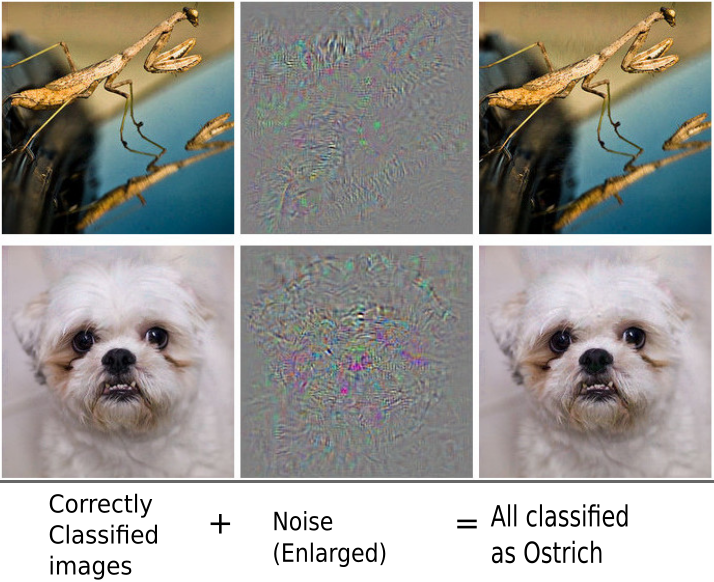
\includegraphics[width=0.5\linewidth, height=0.44\textheight]{img/adv_ex}
	\caption[Examples generated on Alexnet]{Examples generated on Alexnet using GB\protect\footnotemark}
	\label{fig:advex}
\end{figure}
\footnotetext{{\tiny Szegedy, Christian, et al. “Intriguing properties of neural networks.”(2013)}}

\end{frame}

\subsection{Fast gradient sign method}
\begin{frame}
\frametitle{Fast gradient sign method}
$$x_{adv} = x + \epsilon Sign(\nabla_xJ(\theta,x,y))$$
where $x$ is the gradient of the models loss function with respect to the original input pixel vector $x, y$ is the true label vector for $x$ and $\theta$ is the model parameter vector.
\begin{figure}
	\centering
	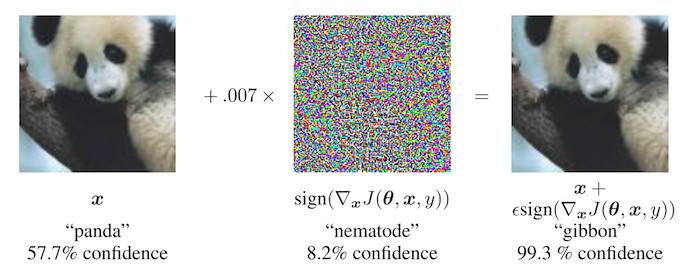
\includegraphics[width=0.93\linewidth, height=0.43\textheight]{img/adversarial-panda}
	\caption{NN predicts Gibbon for a perturbed panda image\protect\footnotemark}
	\label{fig:adversarial-panda}
\end{figure}
\footnotetext{{\tiny Goodfellow et al. “Explaining and harnessing adversarial examples.”(2014)}}
\end{frame}

\subsection{1-pixel attack}
\begin{frame}
\frametitle{Changing a single pixel}
Uses \textbf{differential evolution} to find out which pixel is to be changed and how.
\begin{figure}
	\centering
	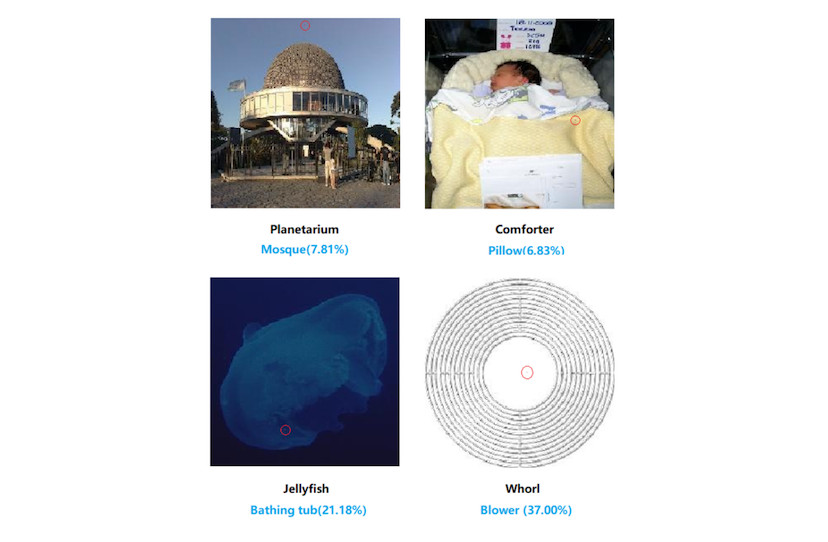
\includegraphics[width=0.8\linewidth,height=0.6\textheight]{img/adversarial-1pixel}
	\caption{Changing a single pixel (marked with circles) to deceive a NN to predict the wrong class instead of the original class.\protect\footnotemark}
	\label{fig:adversarial-1pixel}
\end{figure}


\footnotetext{{\tiny Su et al. “One pixel attack for fooling deep neural networks.”(2019).}}
\end{frame}

\subsection{Adversarial Patch}
\begin{frame}
\frametitle{Adversarial Patch}
Replaces a part of the image with a patch that can take on any shape.

\begin{figure}
	\centering
	\includegraphics[width=1.\linewidth,height=0.52\textheight]{img/adversarial-toaster}
	\caption{Changing a single pixel (marked with circles) to deceive an NN to predict the wrong class instead of the original class.\protect\footnotemark}
	\label{fig:adversarial-patch}
\end{figure}

\footnotetext{{\tiny Brown, Tom B., et al. “Adversarial patch.(2017)}}
\end{frame}

\subsection{Robust adversarial examples}
\begin{frame}
\frametitle{Robust adversarial examples}
\begin{itemize}
	\item[o] Adversarial over transformations (rotation, zoom in) unlike other methods such as FGM.
	\item[o] Expectation Over Transformation (EOT) algorithm.
\end{itemize}

\begin{figure}
	\centering
	\includegraphics[width=0.85\linewidth,height=0.5\textheight]{img/adversarial-turtle}
	\caption{3D-printed turtle that was designed to look like a rifle to a deep NN\protect\footnotemark}
	\label{fig:adversarial-turtle}
\end{figure}

\footnotetext{{\tiny Athalye, Anish, and Ilya Sutskever. “Synthesizing robust adversarial examples.” (2017)}}
\end{frame}

\subsection{Black Box Attacks}
\begin{frame}
\frametitle{Black Box Attacks}
\begin{itemize}
	\item[o] No internal model information required and no access to the training data. \pause
	\item[o] Zero access to model gradient \pause
	\item[o] A surrogate model is trained to approximate the decision boundaries of the black box model, \pause
	\item[o] Can be used to attack machine learning models on cloud platforms with open api access\protect\footnotemark \pause
	\item[o] Although, Knowledge of domain of input is required \pause
\end{itemize}

\footnotetext{{\tiny Papernot, Nicolas, et al. “Practical black-box attacks against machine learning.”(2017)}}
\end{frame}

\section{Coding Session}
\begin{frame}
\frametitle{}
\begin{center}
	\includegraphics[width=0.7\linewidth]{img/let_me_code}
\end{center}

\end{frame}

\section{Combating adversarial examples}
\begin{frame}
\frametitle{Combating adversarial examples}

AEs can be Model-agnostic.

Methods used to combat adversarial examples include\protect\footnotemark;
\begin{itemize}
	\item[1] Adversarial training - iterative retraining of the classifier with adversarial examples \pause
	\item[2] Learning invariant transformations of the features or robust optimization (regularization) \pause
	\item[3] Use of multiple classifiers instead of just one and have them vote the prediction (ensemble) \pause
\end{itemize}
{\small Lot's of research ongoing in this field of Adversarial and ML security.}

\footnotetext{{\tiny https://christophm.github.io/interpretable-ml-book/adversarial.html}}
\end{frame}

\section{Conclusion}
\begin{frame}
\frametitle{Conclusion}
\begin{itemize}
	\item[o] The threats of adversarial examples are real and potent.
	\item[o] These attacks are not limited to computer-vision but span other areas of ML such as NLP, Reinforcement Learning, Speech Recognition e.t.c.
	\item[o] Increasing development in this field (but with equivalent sophistication in attack methods).
\end{itemize}
 
Think of the many different types of spam emails that are constantly evolving (image spam, header masking etc).
\end{frame}

\begin{frame}
\frametitle{}
\begin{center}
	\textbf{{\Huge tHANK yOU}}
\end{center}
\begin{center}
	\includegraphics[width=0.3\linewidth]{img/emoticon-and-smiley-black-white-emoji-clipart-cool}
	{\Large for staying awake}
\end{center}

\end{frame}

\end{document}